%\documentclass[handout]{beamer}
\documentclass{beamer}

\usepackage{amsmath,amsfonts,amssymb,graphicx} 
\usefonttheme[onlymath]{serif}
% use article-like math letters, from http://tex.stackexchange.com/questions/34265/how-to-get-beamer-math-to-look-like-article-math


\newcommand\bi{\begin{itemize}}
\newcommand\ei{\end{itemize}}
\newcommand\simMC{\stackrel{\scriptscriptstyle{MC}}{\sim}}


% from genPomp ms
\newcommand\T{\mathbb{T}}
\newcommand\transmission{\mathcal{T}}
\newcommand\observation{\mathcal{G}}
\newcommand\observationTree{genetic tree}
\newcommand\descendents{h}
\newcommand\sequenceLabel{q}
\newcommand\tInit{t_{0}}
\newcommand\tRoot{t_{\mathrm{root}}}
\newcommand\tEnd{t_{\mathrm{end}}}
\newcommand{\circled}[1]{
  \kern-0.4em \raisebox{.1pt}{\textcircled{\raisebox{-.9pt} {#1}}}
}

\usepackage{natbib}
\usepackage{url}
\usepackage{ulem}
\renewcommand\emph[1]{{\it #1}} % the ulem package redefines \emph
\renewcommand\em{\it} % the ulem package redefines \emph

\usepackage{xcolor}
\definecolor{olive}{rgb}{0.3, 0.4, .1}
\definecolor{dgreen}{rgb}{0.,0.6,0.}
\definecolor{gold}{rgb}{1.,0.84,0.}
\definecolor{JungleGreen}{cmyk}{0.99,0,0.52,0}
\definecolor{BlueGreen}{cmyk}{0.85,0,0.33,0}
\definecolor{RawSienna}{cmyk}{0,0.72,1,0.45}
\definecolor{Magenta}{cmyk}{0,1,0,0}

\usepackage{graphicx} % Allows including images
%\usepackage{booktabs} % Allows the use of \toprule, \midrule and \bottomrule in tables
\mode<presentation> {

\usetheme{Madrid}

%%\setbeamertemplate{footline}[frame number]
\setbeamertemplate{footline}{
  \hfill%
  \usebeamercolor[fg]{page number in head/foot}%
  \usebeamerfont{page number in head/foot}%
  \setbeamertemplate{page number in head/foot}[framenumber]%
  \usebeamertemplate*{page number in head/foot}\kern1em\vskip2pt%
}

\setbeamertemplate{navigation symbols}{} 

}

\newcommand\myemph[1]{{\textbf{#1}}}
\newcommand\enumerateSpace{\hspace{2mm}}
\usepackage{amssymb}
\newenvironment {myitemize} {
                 \begin{list}{\textcolor{black}{$\bullet$} \hfill}
%                 \begin{list}{\textcolor{blue}{{\small{$\blacktriangleright$}}} \hfill}
                 {\setlength{\labelwidth}{0.3 cm}
                  %\setlength{\leftmargin}{0em}
                  \setlength{\leftmargin}{0.15cm}
                  \setlength{\itemindent}{0.15cm}
                  \setlength{\labelsep}{0cm}
                  \setlength{\parsep}{0.2 ex}
%                  \setlength{\itemsep}{0.25 cm}
                  \setlength{\itemsep}{1 mm}
%                   \setlength{\itemsep}{0.0 cm}
      \setlength{\topsep}{0.0cm}}} %space between title and 1st item
   {\end{list}}

\newcommand\MainFigureBmScaling{1}
\newcommand\MainFigureMeaslesScaling{2}
\newcommand\MainFigureMeaslesSlice{3}

%\newcommand\SuppFigureMeaslesSharedSlice{\eic{TODO}}

\newcommand\SuppSecGeneralization{S1}
\newcommand\SuppSecThmI{S3}
\newcommand\SuppSecThmII{S4}
\newcommand\SuppSecMemoryEfficient{S10}
\newcommand\SuppSecAdaptedSimulation{S2}
\newcommand\SuppSecBM{S5}
\newcommand\SuppSecMeasles{S6}
\newcommand\SuppSecMeaslesNbhd{S7}
\newcommand\SuppSecMeaslesGammaSlice{S8}
%\newcommand\SuppSecMeaslesReducedNoise{S9}
\newcommand\SuppSecLorenz{S9}
%\newcommand\SuppSecMeaslesIJ{S11}

%\newcommand\AssumptionBivb{\ref{B:unconditional:mix}(b)}
%\newcommand\AssumptionBiva{\ref{B:unconditional:mix}(a)}
\newcommand\comma{{\hspace{-0.25mm},\hspace{-0.2mm}}}
\newcommand\termStart{\dagger}
%\newcommand\termStart{\circ}

\newcommand\amplitude{a}
\newcommand\meanBeta{{\bar\beta}}
\newcommand\cohort{c}
\newcommand\birth{b}


%\title{Locally weighted island filters for partially observed spatiotemporal systems}

\title{Island filters for partially observed spatiotemporal systems}


%%%%%%%%%%%%%%%% START OF USER DEFINITIONS %%%%%%%%%%%%%%%5

\newcommand\siOnly[1]{} %% redefined for the supplement
\newcommand\msOnly[1]{#1} %% redefined for the supplement

%\newcommand\tif{\mathrm{tif}}
\newcommand\inputSpace{\rule[-1.5mm]{0mm}{4.7mm}}
\newcommand\firstLineSpace{\rule[0mm]{0mm}{4mm}}
\newcommand\lastLineSpace{\rule[-2.5mm]{0mm}{4mm}}

\newcommand\gravity{G}

\newcommand\AIRSIF{ASIF-IR}
\newcommand\TIF{BIF}
\newcommand\centersum{\Delta}
\newcommand\mediumint{\resizebox{2.8mm}{!}{$\displaystyle \int$}}
%\newcommand\Bsize{|B|}
\newcommand\Bsize{b}
%\newcommand\UnitSet{\mathbb{U}}
%\newcommand\TimeSet{\mathbb{N}}
\newcommand\TimeSet{\mbox{TimeSet should now be ObsTimeSet or ProcTimeSet}}
\newcommand\UnitSet{1{\mycolon}\Unit}
\newcommand\ObsTimeSet{1{\mycolon}\Time}
\newcommand\ProcTimeSet{0{\mycolon}\Time}
%\newcommand\spaceTime{\mathbb{S}}
\newcommand\spaceTime{\UnitSet\times\ObsTimeSet}
%\newcommand\unitTimeSubset{\mathbb{C}}
\newcommand\unitTimeSubset{B}
%\newcommand\adapted{\rho}
\newcommand\adapted{\gamma}
\newcommand\myeqref[1]{[\ref{#1}]}
\newcommand\tif{{}}
\newcommand\girf{\mathrm{girf}}
\newcommand\gir{G}
\newcommand\altAltTime{m}


\newcounter{wwii}
\setcounter{wwii}{1}
\newcommand\wwiiStep{\makebox[8mm][l]{\arabic{wwii}.}\stepcounter{wwii}}
\newcounter{wwiiResample}
\newcounter{wwiiAncestor}
\newcounter{wwiiPredict}
\newcounter{wwiiFilter}

\newcounter{asii}
\setcounter{asii}{1}
\newcommand\asiiStep{\makebox[8mm][l]{\arabic{asii}.}\stepcounter{asii}}
\newcounter{girasif}
\setcounter{girasif}{1}
\newcommand\girasifStep{\makebox[8mm][l]{\arabic{girasif}.}\stepcounter{girasif}}
\newcounter{asiiResample}
\newcounter{asiiAncestor}
\newcounter{asiiPredict}
\newcounter{asiiFilter}
\newcounter{girasifResample}
\newcounter{girasifAncestor}
\newcounter{girasifPredict}
\newcounter{girasifFilter}


% package used by default for Overleaf
%\usepackage[utf8]{inputenc}

%% code macros
%\newcommand\slot[1]{\code{#1}}
%\newcommand\class[1]{class `\code{#1}'}
\newcommand\code[1]{\texttt{#1}}
\usepackage{url}

\newcommand\W{W}
\newcommand\V{V}
\newcommand\ASindex{[\Unit]}
\newcommand\simulation{\mathrm{sim}}

%\renewcommand\baselinestretch{1.3}
%\usepackage{showkeys}
%\usepackage[numbers,sort&compress]{natbib}
%\bibliographystyle{apalike}

%\usepackage{natbib}
%\bibliographystyle{plainnat}
%\bibliographystyle{dcu}
%\usepackage{url}

\newcommand\pstep[1]{{\bf #1}}
\newcommand\qsp{\rule{0mm}{1mm}\hspace{4mm}}
\newcommand\plusStrut{\rule{0mm}{1.2mm}}

%% basic POMP definitions
\newcommand\Xspace{{\mathbb X}}
\newcommand\Yspace{{\mathbb Y}}
%\newcommand\Thetaspace{{\Theta}}
\newcommand\Thetaspace{\R^{\Thetadim}}
\newcommand\Xunitspace{{\scriptsize{\mathcal X}}}
\newcommand\Yunitspace{{\tiny{\mathcal Y}}}
\newcommand\hatTheta{\widehat{\Theta}}
\newcommand\Xdim{{\mathrm{dim}}(\Xspace)}
\newcommand\Ydim{{\mathrm{dim}}(\Yspace)}
%\newcommand\Thetadim{{\mathrm{dim}}(\Thetaspace)}
\newcommand\Thetadim{P}
\newcommand\thetadim{p}
\newcommand\timeSet{{\mathbb T}}
\newcommand\data[1]{#1^*}

\newcommand\unitSpecific{\hspace{0.1mm}\mathrm{us}}
\newcommand\shared{\hspace{0.15mm}\mathrm{sh}}

%% for particle filters
\newcommand\unit{u}
\newcommand\altUnit{\tilde u}
\newcommand\Unit{U}
\newcommand\rep{i}
\newcommand\altIsland{\tilde i}
\usepackage[mathscr]{euscript}
\newcommand\Rep{\mathcal{I}}
\renewcommand\time{n}
\renewcommand\vec[1]{\boldsymbol{#1}}
\newcommand\altTime{\tilde n}
\newcommand\Time{N}
\newcommand\Np{J}
\newcommand\np{j}
\newcommand\altNp{k}
\newcommand\altAltNp{\tilde j}
\newcommand\resampleIndex{r}
\newcommand\unitWeight{w}


%% for ASIF and HIPPIE
\newcommand\IF{\mathrm{A}}  % adapted simulation
\newcommand\IP{\mathrm{P}}  % adapted proposal
%\newcommand\GR{\mathrm{GR}}  % GIR resample 
%\newcommand\GP{\mathrm{GP}}  % GIR proposal 
\newcommand\GR{\mathrm{IR}}  % intermediate resample 
\newcommand\GP{\mathrm{IP}}  % intermediate proposal 
\newcommand\resample{\mathrm{R}} % this would have been F before
\newcommand\proposal{\mathrm{P}} 
\newcommand\LCP{\mathrm{P}}  % local prediction 
\newcommand\LCF{\mathrm{F}}  % local filter 

%% for GIR
%\newcommand\Lookahead{L}
%\newcommand\lookahead{\ell}
\newcommand\Ninter{S} %% number of intermediate timepoints
\newcommand\ninter{s}
%\newcommand\Nguide{K} %% number of lookahead particles
%\newcommand\nguide{k}
%\newcommand\lookaheadEnd{\time\oplus \Lookahead}
%\newcommand\lookaheadEnd{\min(\time+\Lookahead,\Time)}
\newcommand\guideFunc{g}
%\newcommand\VtoTheta{{\overleftarrow{V}}}
%\newcommand\thetaToV{{\overrightarrow{V}}}
%\newcommand\VtoTheta{{\overline{V}}}
%\newcommand\thetaToV{\underline{V}}
%\newcommand\thetaToV[1]{\stackrel{\rightarrow}{\mathrm{v}}_{\hspace{-0.5mm}#1}\!}
%\newcommand\VtoTheta[1]{\stackrel{\leftarrow}{\mathrm{v}}_{\hspace{-0.5mm}#1}\!}
\newcommand\thetaToV{\stackrel{\rightarrow}{\mathrm{v}}\!}
\newcommand\VtoTheta{\stackrel{\leftarrow}{\mathrm{v}}\!}
%\newcommand\thetaToV[1]{\stackrel{\rightarrow}{\mathrm{v}_{#1}}\!}
%\newcommand\VtoTheta[1]{\stackrel{\leftarrow}{\mathrm{v}_{#1}}\!}
\newcommand\npgir{\np}
\newcommand\Npgir{\Np}
\newcommand\Nguide{G}

%% for all iterated filtering algorithms
\newcommand\Nit{M}
\newcommand\nit{m}


%% customized math macros
\newcommand\prob{\mathbb{P}}
\newcommand\E{\mathbb{E}}
\newcommand\dd[1]{\mathrm{d}{#1}}
\newcommand\given{{\,\vert\,}}
\newcommand\equals{{{\,}={\,}}} 
\newcommand\myequals{\hspace{0.5mm}{=}\hspace{0.5mm}}
\newcommand\myto{{\;:\;}}
\newcommand\seq[2]{{#1}\!:\!{#2}}
\newcommand\mydot{{\,\cdot\,}}
\newcommand\cp[2]{N_{\mathrm{#1}\mathrm{#2}}}
\newcommand\giventh{{\hspace{0.5mm};\hspace{0.5mm}}}
%\newcommand\normal{{\mathrm{Normal}}}
\newcommand\normal{\mathcal{N}}
\newcommand\argequals{{\,=\,}}
\newcommand\lags{c}
\newcommand\maxlag{\overline{c}}
\newcommand\nlfList{C}
\newcommand\bigO{\mathcal{O}}
\newcommand\loglik{\lambda}
\newcommand\loglikMC{\MC{\loglik}}
\newcommand\R{\mathbb{R}}
\newcommand\param{\,;}
\newcommand\mycolon{{\hspace{0.6mm}:\hspace{0.6mm}}}
\newcommand\MC[1]{#1^{\,\mbox{\tiny MC}}}
%\newcommand\EMC{\MC{\E}}
\newcommand\EMC{{\E}}
\newcommand\Var{\mathrm{Var}}
\newcommand\var{\Var}
\newcommand\Cov{\mathrm{Cov}} 
\newcommand\cov{\Cov}
\newcommand\iid{\mathrm{iid}}
%\newcommand\dist{\mathrm{dist}}
\newcommand\dist{d}
\newcommand\transpose{\top}

\newcommand\gnsep{,}

\def\lik{L}
\def\loglik{\ell}

%% THEOREM-LIKE ENVIRONMENTS
\usepackage{amsthm}
\newtheorem{prop}{Proposition}
%\newtheorem{theorem}{Theorem}
%\newtheorem{lemma}{Lemma}
%\newtheorem{example}{Example}
\newtheorem{remark}{Remark}
\newtheorem{cor}{Corrolary}
%\newtheorem{fact}{Fact}  
\newtheorem{assumption}{Assumption}
\newtheorem{assumptionB}{Assumption}
\newtheorem{procedure}{Procedure}
\renewcommand\theassumption{A\arabic{assumption}}
\renewcommand\theassumptionB{B\arabic{assumptionB}}

%\usepackage{float}
%\floatstyle{ruled}
%\newfloat{textbox}{t}{tbx}
%\floatname{textbox}{Box}
%\renewcommand\thetextbox{\arabic{textbox}}


%% FOR PSEUDOCODE SETUP
\newcommand\mystretch{\rule[-2mm]{0mm}{5mm} }   
\newcommand\asp{\hspace{4mm}}

%%%%%%%%%%%%%%%% END OF USER DEFINITIONSS %%%%%%%%%%%%%%%5


\newcommand\PartOfBoundOffDiagonal{3\efourB+4(K + \dmax)\,\efive}
\newcommand\boundOffDiagonal{\efourA + \PartOfBoundOffDiagonal}
\newcommand\K{K^\prime}
\newcommand\ThmOneVarBound{Q^{4b} \, \Unit\Time  \big(\altb + \etwo \, (\Unit\Time-\altb) \big)}


\newcommand\BvConstant{\mathcal{C}_0}
\newcommand\dmax{d_{\max}}
\newcommand\boundLemma{\efourB+(K+d_{\unit,\time})\efive}
\newcommand\boundLemmaUniform{\efourB+(K+\dmax)\efive}


%\newcommand\altB{\tilde{B}}
\newcommand\altB{C}
%\newcommand\el{\epsilon_\ell}
\newcommand\el{\epsilon}   %%% epsilon for Thm 1
%\newcommand\eone{\epsilon_1}
%\newcommand\eone{\epsilon^{}_{\!\mathrm{\ref{A1}}}}
\newcommand\eone{\epsilon^{}_{\!\mathrm{A1}}}
%\newcommand\eone{\epsilon^{A}_{1}}
%\newcommand\etwo{\epsilon^{}_{\!\mathrm{\ref{A:unconditional:mix}}}}
\newcommand\etwo{\epsilon^{}_{\!\mathrm{A4}}}
%\newcommand\altb{\tilde{b}}
\newcommand\altb{c}
\newcommand\Ai{
\begin{assumption}\label{A1}
There is an $\eone>0$ and a collection of neighborhoods $\{B_{\unit\comma\time}\subset A_{\unit\comma\time}, \unit\in 1\mycolon\Unit,\time\in 1\mycolon\Time\}$ such that, for all  $\unit$, $\time$, $\Unit$, $\Time$,  any  bounded real-valued function $|h(x)|\le 1$, and any value of $x_{B^c_{\unit\comma\time}}$, 
%\begin{equation}
\begin{eqnarray}
\nonumber
&& \hspace{-12mm} \Bigg| \int h(x_{\unit\comma\time}) f_{X_{\unit\comma\time}|Y_{B_{\unit\comma\time}},X_{B^c_{\unit\comma\time}}}(x_{\unit\comma\time}\given  \data{y}_{B_{\unit\comma\time}}, x_{B^c_{\unit\comma\time}}) \, dx_{\unit\comma\time}
\\
\siOnly{\label{eq:weak_coupling2}}
\msOnly{\nonumber}
&& \hspace{-3mm} - \int h(x_{\unit\comma\time})f_{X_{\unit\comma\time}|Y_{B_{\unit\comma\time}}}(x_{\unit\comma\time}\given \data{y}_{B_{\unit\comma\time}})
\, dx_{\unit\comma\time}
\Bigg| \hspace{1mm} < \hspace{1mm} \eone.
%\end{equation}
\end{eqnarray}
\end{assumption}
}

\newcommand\Aii{
\begin{assumption}\label{A1b}
For the collection of neighborhoods in Assumption~\ref{A1}, with $B^+_{\unit\comma\time}=B^{}_{\unit\comma\time}\cup (\unit,\time)$, there is a constant $\Bsize$, depending on $\eone$ but not on $\Unit$ and $\Time$, such that
\begin{equation}
\nonumber
\sup_{\unit\in 1:\Unit, \, \time\in 1:\Time} \big| B^+_{\unit\comma\time}\big| \le \Bsize.
\end{equation}
\end{assumption}
}

\newcommand\Aiii{
\begin{assumption}\label{A2}
There is a constant $Q$ such that, for all $\unit$ and $\time$, $\Unit$ and $\Time$,
\begin{equation}
\nonumber
Q^{-1} <f_{Y_{\unit\comma\time}|X_{\unit\comma\time}}(\data{y}_{\unit\comma\time}\given x_{\unit\comma\time}) < Q
\end{equation}
\end{assumption}
}

\newcommand\Aiv{
  \begin{assumption}\label{A:unconditional:mix}
    There exists $\etwo > 0$ such that the following holds.
    For each $\unit, \time$, a set $\altB^{}_{\unit\comma\time} \subset (1\mycolon U)\times(0\mycolon N)$ exists such that $(\altUnit, \altTime) \notin \altB_{\unit\comma\time}$ implies $B_{\unit\comma\time}^+ \cap B_{\altUnit\comma\altTime}^+ = \emptyset$ and
      \begin{equation} 
\siOnly{\label{eq:A:unconditional:mix}}
\msOnly{\nonumber}
        \big| f_{X_{B^{+}_{\altUnit\comma\altTime}}|X^{}_{B^{+}_{\unit\comma\time}}} - f_{X_{B^{+}_{\altUnit\comma\altTime}}} \big|
        < \etwo \, f_{X_{B^{+}_{\altUnit\comma\altTime}}}
      \end{equation}
      Further, there is a uniform bound $|\altB_{\unit\comma\time}| \le \altb$.
\end{assumption}
}

\newcommand\TheoremI{
\begin{theorem}  \label{thm:tif}
Let $\MC{\loglik}$ denote the Monte Carlo likelihood approximation constructed by {\TIF}.
Consider a limit with a growing number of islands, $\Island\to\infty$, and suppose assumptions~\ref{A1},~\ref{A1b} and~\ref{A2}.
There are quantities $\el(\Unit,\Time)$ and $V(\Unit,\Time)$, with bounds $|\el|<\eone Q^{2}$ and $V < Q^{4\Bsize} \, U^2 N^2$, such that
\begin{equation}
\label{th1:lik:bound}
\Island^{1/2}\big[ \MC{\loglik}-\loglik-\el\Unit\Time \big]  \xrightarrow[\Island \rightarrow \infty]{d} \normal\big[0,V\big],
\end{equation}
where $\xrightarrow[\Island \rightarrow \infty]{d}$ denotes convergence in distribution and $\normal[\mu,\Sigma]$ is the normal distribution with mean $\mu$ and variance $\Sigma$.
If additionally Assumption~\ref{A:unconditional:mix} holds, we obtain an improved variance bound
\begin{equation}
\label{th1:lik:bound2}
V < \ThmOneVarBound.
\end{equation}
\end{theorem}
}


%%% 2222222222222222222222


%\newcommand\ethree{\epsilon^{}_{\mathrm{\ref{B1}}}}
\newcommand\ethree{\epsilon^{}_{\mathrm{B1}}}
%\newcommand\efourA{\epsilon^{}_{\mathrm{\ref{B:unconditional:mix}}}}
\newcommand\efourA{\epsilon^{}_{\mathrm{B4}}}
%\newcommand\efourB{\epsilon^{}_{\mathrm{\ref{B:temporal:mix}}}}
\newcommand\efourB{\epsilon^{}_{\mathrm{B5}}}
%\newcommand\efive{\epsilon^{}_{\mathrm{\ref{B:girf}}}}
\newcommand\efive{\epsilon_{\mathrm{B6}}}

\newcommand\Bi{

\begin{assumptionB}\label{B1}
  There is an $\ethree>0$ and a collection of neighborhoods $\{B_{\unit\comma\time}\subset A_{\unit\comma\time}, \unit\in 1\mycolon\Unit,\time\in 1\mycolon\Time\}$ such that the following holds for all $\unit$, $\time$, $\Unit$, $\Time$, and any bounded real-valued function $|h(x)|\le 1$\emph{:} if we write $A=A_{u,n}$, $B=B_{u,n}$, $f_{A}(x_A) = f_{Y_{A}|X_{A}}(\data y_{A}|x_A)$, and $f_{B}(x_B) = f_{Y_{B}|X_{B}}(\data y_{B}|x_B)$,
%\begin{equation}
\begin{eqnarray}
\nonumber
%\label{asif:eq:weak_coupling2}
&&\hspace{-7mm}
\left| 
\int \hspace{-1mm} h(x)
\left\{
\frac{
  \E_{g} \! \big[ 
    f_{A}\big(X_{A}^P\big) f_{X_{u,n}|X_{A^{[n]}},\vec X_{n-1}} \big(x | X_{A^{[n]}}^P, \vec X_{n-1}\big) 
  \big]
} {
  \E_{g} \! \big[f_A\big(X_A^P\big)\big]
} - 
\right.
\right.
\\
\nonumber
&& 
\siOnly{\hspace{20mm}}
\hspace{-6.5mm} 
% - \hspace{-1mm} 
\siOnly{\hspace{2mm}}
\left.
\left.
\frac{
  \E_{g} \! \big[
    f_{B}\big(X_{B}^P\big) f_{X_{u,n}|X_{B^{[n]}},\vec X_{n-1}}\big(x | X_{B^{[n]}}^P, \vec X_{n-1}\big) \big] 
} {
  \E_{g} \! \big[f_B\big(X_B^P\big)\big]
} 
\!
\right\}
\!
dx
\right| \hspace{0mm} < \hspace{0mm} \ethree.
%\end{equation}
\end{eqnarray}
\end{assumptionB}
}

\newcommand\Bii{
\begin{assumptionB}\label{B1b}
The bound $\sup_{\unit\in 1:\Unit,\time\in 1:\Time} \big| B^+_{\unit\comma\time}\big| \le \Bsize$ in Assumption~\ref{A1b} applies for the neighborhoods defined in Assumption~\ref{B1}. 
This also implies there is a finite maximum temporal depth for the collection of neighborhoods, defined as
\begin{equation}
\nonumber
\dmax=\sup_{(\unit,\time)}\hspace{1mm} \sup_{(\altUnit,\altTime)\in B_{\unit,\time}}|\time-\altTime|.
\end{equation}
\end{assumptionB}
}

\newcommand\Biii{
\begin{assumptionB}\label{B2} Identically to Assumption~\ref{A2}, 
$Q^{-1} <f_{Y_{\unit\comma\time}|X_{\unit\comma\time}}(\data{y}_{\unit\comma\time}\given x_{\unit\comma\time}) < Q$.
\end{assumptionB}
}

\newcommand\BivA{
\begin{assumptionB}\label{B:unconditional:mix}
Define $g_{{X}_{A}|{X}_{B}}$ via \myeqref{eq:g}.
Suppose there is an $\efourA$ such that the following holds.
For each $\unit, \time$, a set $\altB^{}_{\unit\comma\time} \subset (1\mycolon U)\times(0\mycolon N)$ exists such that $(\altUnit, \altTime) \notin \altB_{\unit\comma\time}$ implies $B_{\unit\comma\time}^+ \cap B_{\altUnit\comma\altTime}^+ = \emptyset$ and
%      \begin{eqnarray} 
%\label{eq:B:unconditional:mix:1}
\begin{equation}
\nonumber
\big| 
   g^{}_{{X}^{P}_{B^{}_{\altUnit\comma\altTime}}{X}^{P}_{B^{}_{\unit\comma\time}}} 
   - g^{}_{{X}^{P}_{B^{}_{\altUnit\comma\altTime}}} \, g^{}_{{X}^{P}_{B^{}_{\unit\comma\time}}} 
\big|
<
%&\hspace{-3mm}<\hspace{-3mm} & 
%\\
%&&\hspace{-30mm}
(1/2) \, \efourA \, \,  g^{}_{{X}^{P}_{B^{}_{\altUnit\comma\altTime}}} \, g^{}_{{X}^{P}_{B^{}_{\unit\comma\time}}}
%\\
%\label{eq:B:unconditional:mix:2}
\end{equation}
\begin{eqnarray}
\nonumber
\big|
g^{}_{X^P_{B^{}_{\altUnit\comma\altTime}}|\vec{X}_{0:\Time}} 
\, g^{}_{X^P_{B^{}_{\unit\comma\time}}|\vec{X}_{0:\Time}} 
-
g^{}_{X^P_{B^{}_{\altUnit\comma\altTime}},X^P_{B^{}_{\unit\comma\time}}|\vec{X}_{0:\Time}}
\big|
&&
%&\hspace{-3mm}<\hspace{-3mm}& 
\\
\nonumber
%&&\hspace{-30mm}(1/2) \, \efourA \, \, 
&&\hspace{-30mm} < (1/2) \, \efourA \, \, 
 g^{}_{X^P_{B^{}_{\altUnit\comma\altTime}},X^P_{B^{}_{\unit\comma\time}}|\vec{X}_{0:\Time}}
      \end{eqnarray}
      Further, there is a uniform bound $|\altB_{\unit\comma\time}| \le \altb$.
\end{assumptionB}
}
\newcommand\BivB{
\begin{assumptionB}\label{B:temporal:mix}
There is a constant $K$ such that, for any set $D\subset (\UnitSet)\times(n{\mycolon}n-d)$ and for all $\time\ge K+d$, $\vec{x}^{(1)}_{\time-d-K}$, $\vec{x}^{(2)}_{\time-d-K}$, and all $x^{}_{D_n}$,
\begin{eqnarray}
\nonumber
&&\hspace{-6mm} \big|
g^{}_{{X}_{D}|\vec{X}_{\time-d-K}}(x^{}_{D}\given\vec{x}^{(1)}_{\time-d-K})
-
g^{}_{{X}_{D}|\vec{X}_{\time-d-K}}(x^{}_{D}\given\vec{x}^{(2)}_{\time-d-K})
\big|
\\
\nonumber
&& \siOnly{\hspace{10mm}} \hspace{4mm}
< 
\efourB  \,  \,
g^{}_{{X}_{D}|\vec{X}_{\time-d-K}}(x^{}_{D_n}\given\vec{x}^{(1)}_{\time-d-K})
\end{eqnarray}

\end{assumptionB}
}

\newcommand\Bv{
\begin{assumptionB}\label{B:girf}
Let $h$ be a bounded function with $|h(x)|\le 1$. 
Let $\vec{X}^{\GR}_{\time,\Ninter,\np,\island}$ be the Monte Carlo quantity constructed in ASIF-IR, conditional on $\vec{X}^{\IF}_{\time-1,\Ninter,\island}=\vec{x}^{\IF}_{\time-1,\Ninter,\island}$.
There is a constant $\BvConstant(\Unit,\Time,\Ninter)$ such that, for all $\efive^{}>0$ and $\vec{x}^{\IF}_{\time-1,\Ninter,\island}$, whenever the number of particles satisfies $J > \BvConstant(\Unit,\Time,\Ninter)/\efive^{4}$,
\begin{equation}
\nonumber
\hspace{-0.5mm}
\left|  
\, 
  \EMC\Big[ 
    \frac{1}{\Np} \sum_{\np=1}^{\Np} h(\vec{X}^{\GR}_{\time,\Ninter,\np,\island}) 
   \Big] \!
-  \E_g \! \big[h(\vec{X}_\time)\given \vec{X}_{\time-1}=\vec{x}^{\IF}_{\time-1,\Ninter,\island}\big] 
\right| \!
< \efive^{}.
\end{equation}
\end{assumptionB}
}

\newcommand\Bvi{
\begin{assumptionB}\label{B:XG_XA_ind}
For $1\leq \time \leq N$, the Monte Carlo random variable $X^A_{\time,i}$ is independent of $w^M_{\unit,\time,i,j}$ conditional on $X^A_{\time-1,i}$.
\end{assumptionB}
}


\newcommand\TheoremII{
\begin{theorem}  \label{thm:asif}
Let $\MC{\loglik}$ denote the Monte Carlo likelihood approximation constructed by ASIF-IR, or by ASIF since this is the special case of ASIF-IR with $\Ninter=1$.
Consider a limit with a growing number of islands, $\Island\to\infty$, and suppose assumptions~\ref{B1},~\ref{B1b}, \ref{B2}, \ref{B:temporal:mix}, \ref{B:girf} and~\ref{B:XG_XA_ind}. 
Suppose the number of particles $\Np$ exceeds the requirement for~\ref{B:girf}.
There are quantities $\el(\Unit,\Time)$ and $V(\Unit,\Time)$ with $|\el|<
Q^2\ethree + 2 Q^{2\Bsize}\big(\boundLemma\big)$
and $V<Q^{4\Bsize}\Unit^2\Time^2$ 
such that
\begin{equation}
\siOnly{\label{th:asif:lik:bound}}
\msOnly{\nonumber}
\Island^{1/2}
  \big[ 
    \MC{\loglik}-\loglik-\el\Unit\Time 
  \big]  
  \xrightarrow[\Island \rightarrow \infty]{d} 
  \normal\big[ 0,V \big].
\end{equation}
If additionally Assumption~\ref{B:unconditional:mix} holds, we obtain an improved rate of
\begin{equation}
\siOnly{\label{th:asif:lik:bound2}}
\msOnly{\nonumber}
V < Q^{4\Bsize}\Time\Unit
\big\{ c + \big(\boundOffDiagonal \big) \big(\Time\Unit-c\big)
\big\}
\end{equation}
\end{theorem}
}



\begin{document}

\begin{frame}
\begin{center}
  {\Large\bf Inference for metapopulation dynamics}

%% ABSTRACT: Microbial populations can demonstrate highly nonlinear, partially observable, stochastic dynamics. Parameter estimation and model criticism are inferential challenges which are tractable using modern methods applicable to general low-dimensional ecological models. Collections of interacting ecosystems at different locations raise additional challenges associated with high-dimensional Monte Carlo inference. Questions arise about when it is necessary to develop models for dynamic coupling between metapopulations, and if so how to carry out inference in this setting. We seek general-purpose methods that allow scientists to ask and answer questions for metapopulation dynamics in the context of scientifically useful models. We present recent progress and ongoing developments.


\vspace{2mm}

Edward Ionides\\
University of Michigan, Department of Statistics

\vspace{8mm}

% Algorithms \& Computationally Intensive Inference seminar\\
% University of Warwick
\\
% Friday November 26, 2021
\\

\hspace{3mm}

Slides are at \url{https://ionides.github.io/talks/imsi22.pdf}
%% 8:15am EST

\vspace{8mm}

Joint work with\\
Kidus Asfaw, Ning Ning, Joonha Park and Aaron King\\

\end{center}

\end{frame}


\newcommand\challengeSep{\vspace{3mm}}

\begin{frame}{Seven inferential challenges for ecological and epidemiological dynamics}

  \bi
\item 1--6 are from ??
\item 7 is from ??
  \item 1--5 are now fairly well solved
  
\end{frame}

\begin{frame}{Example: Pre-vaccination measles in England \& Wales}

\end{frame}

\begin{frame}{Time series vs Panel data vs Spatiotemporal data}

  \bi
\item Looking at one unit (town) is \myemph{time series analysis}. Joint modeling of a few units (say, 2 or 3) is \myemph{multivariate time series analysis}.

\item Analysis of many time series, while ignoring dynamic interactions, is \myemph{panel data analysis}.

\item Allowing for coupling between units, we get \myemph{spatiotemporal} analysis, also called \myemph{metapopulation analysis}.

  \ei
  
Question: When should we avoid inference for spatiotemporal models? When do we need to do it? How?

\end{frame}

\begin{frame}{Desiderata}

  \begin{itemize}
    \item We want to be able to fit arbitrary dynamic models. The limitations should be our scientific creativity and the information in the data.

    \item In practice, that means using \myemph{plug-and-play} methods which need a simulator from the model but not nice parametric equations.

    \item We want statistically efficient inference, that lets us extract all the information in the data.

    \item In practice, that means using likelihood-based methods.

      \item The iterated particle filtering algorithm IF2, implemented in the R package pomp, enables Masters-level statisticians to carry out such analysis routinely in the time series case \url{}
      \end{itemize}
  \end{frame}



\begin{frame}
  \frametitle{Outline}

  
  \myemph{The curse of dimensionality}. Particle filter (PF) methods are effective for inference on low-dimensional nonlinear partially observed stochastic dynamic systems. They scale exponentially badly.

  \challengeSep
  
  \myemph{Bagged filters}. Combining independent Monte Carlo filters.

  \vspace{1mm}
  
  \begin{myitemize}
  \item Unadapted bagged filter (UBF)
  \item Adapted bagged filter (ABF)
    \item Adapted bagged filter with intermediate resampling (ABF-IR)
  \end{myitemize}

  \challengeSep

  \myemph{Blocked particle filter} (BPF). Theory by \citet{rebeschini15}. Independently proposed by \citet{ng02}.

  \challengeSep

  \myemph{From filtering to inference}. Iterated filtering using stochastically perturbed parameters.

  \challengeSep

  \myemph{Metapopulation dynamics}. Bagged and blocked filters work on collections of weakly coupled populations, in theory and practice.

\end{frame}

\begin{frame}

  \frametitle{What is a SpatPOMP?}

  \myemph{POMP} models are partially observed Markov processes, also known as state space models or hidden Markov models.

  \vspace{6mm}
  
  \myemph{SpatPOMP} models are POMP models with a unit structure.

    \vspace{6mm}
 
  \myemph{Latent Markov process}: $X_{\unit\comma\time}=X_{\unit}(t_\time)$, \hspace{1mm} $\unit\in 1{\mycolon}\Unit$, \hspace{1mm} $\time\in 1{\mycolon}\Time$

    \vspace{6mm}
 
  \myemph{Observation process}: $Y_{\unit\comma\time}$ depends only on $X_{\unit\comma\time}$

    \vspace{6mm}
 
The units could be a metapopulation, say cities in an epidemic model.

\end{frame}


\begin{frame}
\frametitle{$U=40$ units for a coupled measles SEIR model}

\vspace{-2.7mm}

\begin{center}
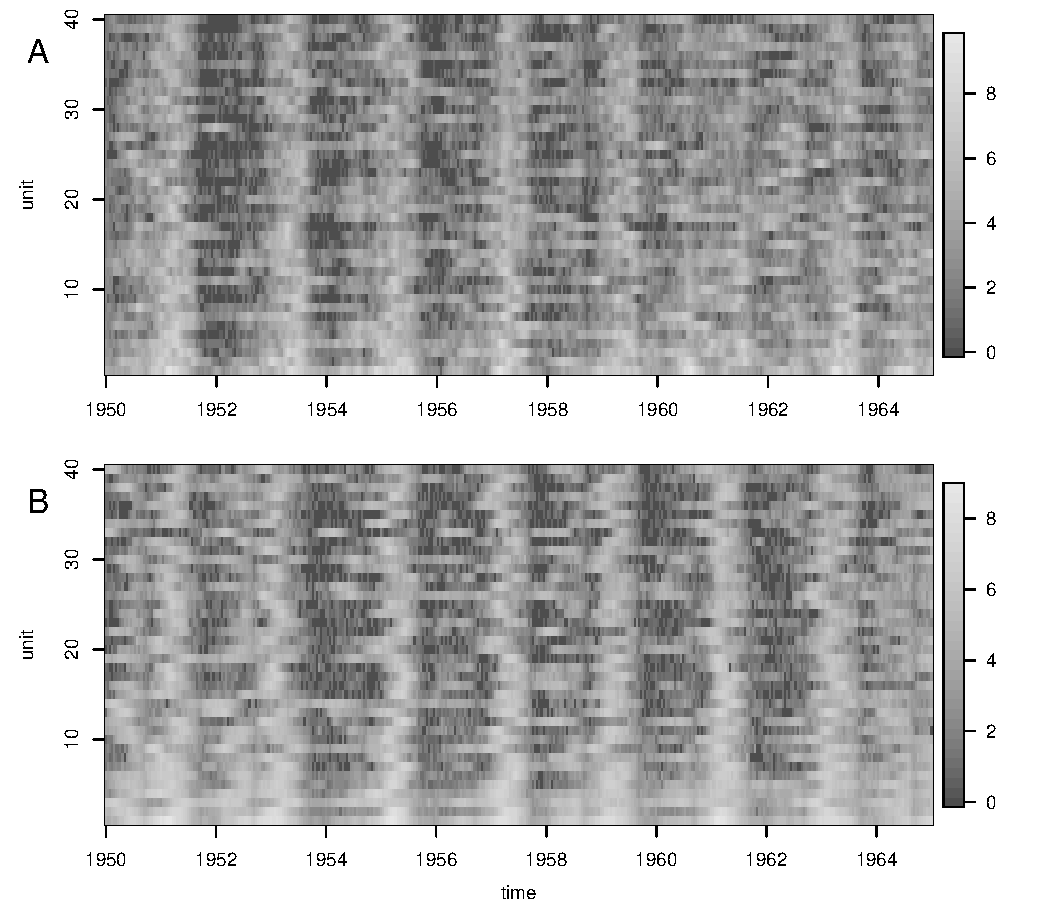
\includegraphics[width=8cm]{slice_image_plot-1.pdf}
\end{center}

\vspace{-3mm}

{\bf A}. Simulated Susceptible-Exposed-Infected-Recovered dynamics coupled with a gravity model (log of biweekly reported cases).

{\bf B}. Measles UK pre-vaccination case reports for the 40 largest cities.




%\end{center}

\end{frame}

\begin{frame}{Particle filter (PF)}

  \begin{columns}
    \begin{column}{0.48\linewidth}
      \begin{center}
      {\bf \textcolor{blue}{Evolutionary analogy}}

      \vspace{5mm}
      
      {\bf Mutation}

      $\downarrow$

      {\bf Fitness}

      $\downarrow$

      {\bf Natural selection}
      
      \end{center}
    \end{column}
     \begin{column}{0.48\linewidth}
      \begin{center}
      {\bf \textcolor{blue}{Particle filter algorithm}}

      \vspace{5mm}
      
      {\bf Predict: stochastic dynamics}

      $\downarrow$

      {\bf Measurement: weight}

      $\downarrow$

      {\bf Filter: resample}
      \end{center}
    \end{column}
  \end{columns}

  \vspace{15mm}
  
    \begin{myitemize}
  \item PF is an evolutionary algorithm with good mathematical properties: an unbiased likelihood estimate and consistent latent state distribution.
  \end{myitemize}

\end{frame}
  
\begin{frame}{Block particle filter (BPF)}

  \begin{columns}
    \begin{column}{0.48\linewidth}
      \begin{center}
      {\bf \textcolor{blue}{Evolutionary analogy}}

      \vspace{5mm}
      
      {\bf Mutation}

      $\downarrow$

      {\bf Fitness\\
      for each chromosome}

      $\downarrow$

      {\bf Natural selection\\
      for each chromosome}

      $\downarrow$

      {\bf Recombine chromosomes}
      
      \end{center}
    \end{column}
     \begin{column}{0.48\linewidth}
      \begin{center}
      {\bf \textcolor{blue}{Block particle filter}}

      \vspace{5mm}
      
      {\bf Predict: stochastic dynamics}

      $\downarrow$

      {\bf Measurement: weight\\
      for each block}

      $\downarrow$

      {\bf Filter: resample\\
      for each block}

      $\downarrow$

      {\bf Recombine blocks}
      \end{center}
    \end{column}
  \end{columns}

  \vspace{10mm}
  
    \begin{myitemize}
    \item Blocks in BPF allow recombination (reassortment of chromosomes in sexual reproduction) in the evolutionary analogy.
\item Blocks are a partition of the spatial units. 
  \end{myitemize}

\end{frame}

\begin{frame}{Anticipated limitations of BPF}

\citet{rebeschini15} proved an asymptotic limit where BPF beats the curse of dimensionality but were modest in their applied hopes since blocks small enough to be practical might give unacceptable bias.

\vspace{8mm}

\begin{myitemize}
\item \textcolor{blue}{``not anticipated to be applicable to real high-dimensional
  problems''}

  \vspace{5mm}
  
\item \textcolor{blue}{``it is far from clear whether this simple algorithm is of immediate practical utility in the most complex real-world applications''}

\end{myitemize}

\vspace{8mm}

Thus we look for algorithms without this weakness which also have provable scalability.

\end{frame}

\newcommand\PPlist{\vspace{2mm}}
\begin{frame}{Plug-and-play methods for implicit models}
  \begin{myitemize}

  \item We address stochastic dynamic models where a simulator is available, but transition densities are not readily accessible.

    \PPlist
    
\item These models have been called implicit \citep{diggle84}.

    \PPlist

  \item An algorithm that uses a simulator but not transition densities is called plug-and-play \citep{breto09,he10}.

        \PPlist

      \item Plug-and-play methods can be applied to implicit models.

            \PPlist

          \item Similar ideas have been called equation-free and likelihood-free.

          \item BPF is plug-and-play.
            
          \item We now consider another scalable simple plug-and-play filter with different strengths and weaknesses to BPF.
            
  \end{myitemize}

\end{frame}

\begin{frame}
  % UBF PSEUDOCODE uuuuuuuuuu
\begin{algorithm}[H]
  \caption{\bf Unadapted bagged filter (UBF).
   }\label{alg:ubf}
  \KwIn{
    simulator for $f_{\myvec{X}_{\time}|\myvec{X}_{\time-1}}(\myvec{x}_{\time}\given \myvec{x}_{\time-1})$ and $f_{\myvec{X}_0}(\myvec{x}_0)$;
    evaluator for $f_{{Y}_{\unit,\time}|{X}_{\unit,\time}}({y}_{\unit,\time}\given {x}_{\unit,\time})$;
    data, $\data{\myvec{y}}_{1:\Time}$;
    number of replicates, $\Rep$;
    neighborhood structure, $B_{\unit,\time}$
  }
\For{$\rep\ \mathrm{in}\ \seq{1}{\Rep}$}{
initialize simulation, $\myvec{X}_{0,\rep} \sim f_{\myvec{X}_0}(\cdot)$
  \;
  \nllabel{alg:ubf:for:n}
\For{$\time\ \mathrm{in}\ \seq{1}{\Time}$}{
simulate,
    $\myvec{X}_{\time,\rep} \sim
      f_{\myvec{X}_{\time}|\myvec{X}_{\time-1}}
      \big( \mydot \given \myvec{X}_{\time-1,\rep}
    \big)$
  \nllabel{alg:ubf:adapted:proposals}
  \;
measurement weights,
  $w^M_{\unit,\time,\rep}=
    f_{Y_{\unit,\time}|X_{\unit,\time}}
    \big (\data{y}_{\unit,\time}\given {X}_{\unit,\time,\rep}
  \big)$
%    for $\unit$ in $\seq{1}{\Unit}$
  \;
prediction weights,
  $w^P_{\unit,\time,\rep}=\prod_{(\tilde \unit,\tilde n)\in B_{\unit,\time}} w^M_{\tilde\unit,\tilde n,\rep}$
%    for $\unit$ in $\seq{1}{\Unit}$
      \nllabel{alg:ubf:adapted:weights}
  \;
  }
}
%conditional log likelihood,
  $\MC{\loglik}_{\unit,\time}= 
    \log\left(
      \sum_{\rep=1}^\Rep w^M_{\unit,\time,\rep}w^P_{\unit,\time,\rep}
    \right)
    -\log\left(
      \sum_{\rep=1}^\Rep w^P_{\unit,\time,\rep}
    \right)$
%  for $\unit$ in $\seq{1}{\Unit}$, $\time$ in $\seq{1}{\Time}$
  \;
\KwOut{
log likelihood estimate, $\MC{\loglik}= \sum_{\time=1}^\Time\sum_{\unit=1}^\Unit \MC{\loglik}_{\unit\comma\time}$\\
}
\end{algorithm}


\end{frame}

\newcommand\BFsep{\vspace{4mm}}

\begin{frame}{Bagged filters}

  \begin{myitemize}

  \item {\bf Bagging} is bootstrap aggregating. The goal is to gain strength from many boostrap replicates.

    \BFsep
    
  \item Simulating from a postulated model is a simple parametric bootstrap.

    \BFsep
    
  \item To obtain scalability, we use local weights to aggregate the bootstrap replicates.

    \BFsep
    
    \item The unadapted bagged filter is a fancy name for a simple algorithm.  We view it a starting point for adapted bagged filters.

      \end{myitemize}
  
\end{frame}

\begin{frame}

  \frametitle{The unadapted bagged filter is not entirely naive}

  \begin{myitemize}

  \item UBF seems naive. Particle filter (PF) method are well known to scale better with $\Time$ than unconditional simulations.

    \vspace{5mm}
    
  \item With modern computers, large numbers of simulations are feasible even when $\Unit$ and $\Time$ are not small.

      \vspace{5mm}

    \item Initially we studied UBF as a theoretical toy, since it is relatively easy to show theoretically that it can beat the curse of dimensionality as $U$ increases, for weakly coupled systems. Then we found it is competitive in practice on some models of interest.
  \end{myitemize}

\end{frame}

\begin{frame}
  \frametitle{Adapted simulation: An easier problem than filtering}

  \begin{myitemize}
  \item
    We aim to make each replicate track the data in a weak sense, easier and more scalable than solving the full filtering problem.

\vspace{3mm}

  \item
    The adapted simulation problem is to draw from
$f_{\vec{X}_{\time}|\vec{Y}_{\time},\vec{X}_{\time-1}}
  \big(
    \vec{x}_{\time}\given \vec{\data{y}}_{\time},\vec{x}_{\time-1}
  \big)$.

\vspace{3mm}

  \item The adapted bagged filter (ABF) algorithm uses importance sampling to carry out adapted simulation on each replicate, with a sample size $\Np$.

    \vspace{3mm}
    
  \item Importance sampling for adapted simulation does NOT beat the curse of dimensionality.
We combine it with intermediate resampling to give scalability.

\vspace{3mm}

    \item ABF calculates the likelihood using the proper weight restricted to a neighborhood.
\end{myitemize}
    
\end{frame}



\begin{frame}

%\setlength\extrarowheight{5pt}
\renewcommand{\arraystretch}{1.2}.
\noindent\begin{tabular}{l}
\hline
{\bf 
{ABF}. Adapted bagged filter.}\inputSpace\\
\hline
%{\bf input:} From Table~1 \inputSpace \\
%\hline
\firstLineSpace
Initialize adapted simulation: $\vec{X}^{\IF}_{0,\rep} \sim f_{\vec{X}_0}(\vec{x}_0)$
\\
For $\time\ \mathrm{in}\ \seq{1}{\Time}$
\\
\asp  Proposals:
    $\vec{X}_{\time,\rep,\np}^{\IP} \sim 
    f_{\vec{X}_{\time}|\vec{X}_{\time-1}} 
    \big( \vec{x}_{\time}\given \vec{X}^{\IF}_{\time-1,\rep}\big)$
\\
\asp Measurement weights:
  $w^M_{\unit,\time,\rep,\np} = 
    f_{Y_{\unit,\time}|X_{\unit\comma\time}} 
    \big (\data{y}_{\unit\comma\time}\given X^{\IP}_{\unit\comma\time,\rep,\np}\big)$
\\
\asp  Adapted resampling weights:
  $w^{\IF}_{\time,\rep,\np} = 
    \prod_{\unit=1}^{\Unit} w^M_{\unit,\time,\rep,\np}$
\\
\asp
      Resampling:
        $\prob\big[\resampleIndex({\rep})=a \big] = w^{\IF}_{\time,\rep,a}
  \Big( 
  \sum_{\altNp=1}^{\Np} w^{\IF}_{\time,\rep,\altNp}
  \Big)^{-1}$
\\
\asp 
$\vec{X}^{\IF}_{\time,\rep} = \vec{X}^{\IP}_{\time,\rep,r(\rep)}$ 
\\
\asp % Prediction weights:
  $w^{\LCP}_{\unit,\time,\rep,\np}= \displaystyle
  \prod_{\altTime=1}^{\time-1}
  \Big[
    \frac{1}{\Np}\sum_{k=1}^{\Np}
    \hspace{1mm}
       \prod_{(\altUnit,\altTime)\in B^{[\altTime]}_{\unit,\time}} 
    \hspace{-1mm}
        w^M_{\altUnit,\altTime,\rep,k}
  \Big] \prod_{(\altUnit,\time)\in B^{[\time]}_{\unit,\time}} 
    \hspace{-1mm}
        w^M_{\altUnit,\time,\rep,\np}$
\\
End for
\\
$\displaystyle \MC{\loglik}_{\unit,\time}= 
\log\Bigg(
\frac{
\sum_{\rep=1}^\Rep \sum_{\np=1}^{\Np} w^M_{\unit,\time,\rep,\np}w^P_{\unit,\time,\rep,\np}
}{
\sum_{\rep=1}^\Rep \sum_{\np=1}^{\Np} w^P_{\unit,\time,\rep,\np}
}
\Bigg)
$
\rule[-8mm]{0mm}{10mm}
\\
\hline
\end{tabular}
\end{frame}


\begin{frame}
\frametitle{Intermediate resampling}



\begin{myitemize}
\item \myemph{Intermediate resampling} splits the time interval between observations into $\Ninter$ subintervals.

\vspace{2mm}

\item Reweighting and/or sampling at each subinterval uses a revised estimate of the anticipated measurement density at the end of the interval called a \myemph{guide function}.

\vspace{2mm}

\item This is applicable to continuous time models.

\vspace{2mm}

\item Intermediate resampling has useful theoretical and empirical properties \citep{delmoral15,park20}.

\vspace{2mm}

\item Intermediate resampling for adapted simulation within ABF gives the ABF-IR algorithm.

\vspace{2mm}

\item Intermediate resampling within PF gives the guided intermediate resampling filter (GIRF) of \citet{park20}, a generalization of the auxiliary particle filter of \citet{pitt99}.
  
\end{myitemize}

\end{frame}


\begin{frame}{A guide function for intermediate resampling}

  \begin{myitemize}

  \item Intermediate resampling with an ideal guide function can beat the curse of dimensionality \citep{park20}.

    \vspace{3mm}
    
  \item  It is consistent for any guide function, but scalability is limited in practice since the ideal guide is generally intractable.

    \vspace{3mm}
    
    \item In practice, we use moment-matching to approximate the ideal guide for Gaussian models. 

      \vspace{3mm}
      
    \item Additional algorithmic parameters:\\

      \vspace{1mm}
      
      number of intermediate timesteps, $\Ninter$ \\
      measurement variance parameterizations, ${\VtoTheta}_{\unit\comma\time}$ and ${\thetaToV}_{\unit\comma\time}$\\
      approximate process and observation mean functions, $\vec{\mu}$ and $h_{\unit\comma\time}$

\vspace{3mm}
      
\item Guided intermediate resampling is plug-and-play: it does not need evaluation of transition densities.

        \end{myitemize}

\end{frame}

  
\begin{frame}

  \resizebox{!}{45mm}{
\noindent\begin{tabular}{l}
\hline
{\bf {ABF-IR}. ABF  with  intermediate resampling.} 
\vspace{0.4mm} \\
\hline
\firstLineSpace
Initialize adapted simulation: $\vec{X}^{\IF}_{0,\rep} \sim f_{\vec{X}_0}(\vec{x}_0)$
\\
For $\time\ \mathrm{in}\ \seq{1}{\Time}$
\\
\asp Guide simulations:
    $\vec{X}_{\time,\rep,\npgir}^{G} \sim 
    f_{\vec{X}_{\time}|\vec{X}_{\time-1}} 
    \big( \vec{x}_{\time}\given \vec{X}^{\IF}_{\time-1,\rep} \big)$
\\
\asp Guide variance: $V_{\unit,\time,\rep}=
      \var \big\{
        h_{\unit\comma\time}\big( {X}_{\unit,\time,\rep,\npgir}^{G}\big), \npgir \mbox{ in } \seq{1}{\Npgir}
      \big\}$ 
\\
\asp $\guideFunc^{\resample}_{\time,0,\rep,\np}=1 \; \; $ and
$\; \vec{X}_{\time,0,\rep,\np}^{\GR}=\vec{X}^{\IF}_{\time-1,\rep}$
\\
\asp For $\ninter  \,\, \mathrm{in} \,\, \seq{1}{\Ninter}$
\\
\asp\asp Intermediate proposals:
        ${\vec{X}}_{\time,\ninter,\rep,\np}^{\GP}
          \sim {f}_{{\vec{X}}_{\time,\ninter}|{\vec{X}}_{\time,\ninter-1}}
          \big(\mydot|{\vec{X}}_{\time,\ninter-1,\rep,\np}^{\GR}\big)$ 
\\
\asp\asp 
        $\vec{\mu}^{\GP}_{\time,\ninter,\rep,\np} 
           = \vec{\mu}\big( \vec{X}^{\GP}_{\time,\ninter,\rep,\np},t_{\time,\ninter},t_{\time} \big)$
\\
\asp\asp      %Measurement variance at skeleton: 
        $V^{\mathrm{meas}}_{\unit,\time,\ninter,\rep,\np}
           = \thetaToV_{\unit}(\theta,\mu^{\GP}_{\unit,\time,\ninter,\rep,\np})$
%\\
           %\asp\asp  %Process variance:
           , \hspace{4mm}
        $V^{\mathrm{proc}}_{\unit,\time,\ninter,\rep}
          = V_{\unit,\time,\rep} \,
          \big(t_{\time}-t_{\time,\ninter}\big) \Big/
          \big(t_{\time}-t_{\time,0}\big)$ 
\\
\asp\asp
%      Moment matching:
        $\theta_{\unit,\time,\ninter,\rep,\np}= 
          \VtoTheta_{\unit}\big(
            V^{\mathrm{meas}}_{\unit,\time,\ninter,\rep,\np} + V^{\mathrm{proc}}_{\unit,\time,\ninter,\rep}, 
            \, \mu^{\GP}_{\unit,\time,\ninter,\rep,\np}
          \big)$
\\
\asp\asp  % Guide function: 
        $
\guideFunc_{\time,\ninter,\rep,\np}=
          \prod_{\unit=1}^{\Unit}
          f_{Y_{\unit,\time}|X_{\unit,\time}}
          \big(
            \data{y}_{\unit,\time}\given \mu^{\GP}_{\unit,\time,\ninter,\rep,\np} \giventh \theta_{\unit,\time,\ninter,\rep,\np} 
          \big)$
\\
\asp\asp Guide weights:
$w^G_{\time,\ninter,\rep,\np}= \guideFunc^{}_{\time,\ninter,\rep,\np}
         \big/ \guideFunc^{\resample}_{\time,\ninter-1,\rep,\np}$
\\
\asp\asp
      Resampling:
        $\prob\big[\resampleIndex({\rep,\np})=a \big] = w^G_{\time,\ninter,\rep,a}
\Big( \sum_{\altNp=1}^{\Np}w^G_{\time,\ninter,\rep,\altNp}\Big)^{-1}$
\\
\asp\asp
        $\vec{X}_{\time,\ninter,\rep,\np}^{\GR}=\vec{X}_{\time,\ninter,\rep,\resampleIndex({\rep,\np})}^{\GP}\; \; $ and
        $\; \guideFunc^{\resample}_{\time,\ninter,\rep,\np}= \guideFunc^{}_{\time,\ninter,\rep,\resampleIndex({\rep,\np})}\,$
\\
\asp
End For
\\
\asp
  Set $\vec{X}^{\IF}_{\time,\rep}=\vec{X}^{\GR}_{\time,\Ninter,\rep,1}$ 
\\ 
\asp Measurement weights:
  $w^M_{\unit,\time,\rep,\npgir} = 
    f_{Y_{\unit,\time}|X_{\unit,\time}} 
    \big (\data{y}_{\unit,\time}\given X^{G}_{\unit,\time,\rep,\npgir} \big)$
\\
\asp % Prediction weights:
  $w^{\LCP}_{\unit,\time,\rep,\npgir}= \displaystyle
  \prod_{\altTime=1}^{\time-1}
  \Big[
    \frac{1}{\Npgir}\sum_{a=1}^{\Npgir}
    \hspace{1mm}
       \prod_{(\altUnit,\altTime)\in B^{[\altTime]}_{\unit,\time}} 
    \hspace{-1mm}
        w^M_{\altUnit,\altTime,\rep,a}
  \Big] \prod_{(\altUnit,\time)\in B^{[\time]}_{\unit,\time}} 
    \hspace{-1mm}
        w^M_{\altUnit,\time,\rep,\npgir}$
\\
End for
\\
$\displaystyle \MC{\loglik}_{\unit,\time}= 
\log\Bigg(
\frac{
\sum_{\rep=1}^\Rep \sum_{\npgir=1}^{\Npgir} w^M_{\unit,\time,\rep,\npgir}w^P_{\unit,\time,\rep,\npgir}
}{
\sum_{\rep=1}^\Rep \sum_{\npgir=1}^{\Npgir} w^P_{\unit,\time,\rep,\npgir}
}
\Bigg)
$
\vspace{1mm}
\\
\hline
\end{tabular}
}
\end{frame}

\begin{frame}
  \frametitle{Software for SpatPOMP models}


  \newcommand\spatpompsep{\vspace{3mm}}
  
  \begin{myitemize}
    
  \item We use the \code{asif}, \code{asifir}, \code{bpfilter}, \code{enkf} and \code{girf} implementations in the  R package \code{spatPomp} \citep{asfaw20github}.

    \spatpompsep
    
\item All these algorithms are plug-and-play. This facilitates implementations applicable to a wide class of models: SpatPOMPs that can be simulated.
   
      \spatpompsep

  \item \code{spatPomp} offers a class `\code{spatPomp}' that extends the `\code{pomp}' class for POMP models in the R package \code{pomp} \citep{king16}.

    \spatpompsep

\item All methods available in \code{pomp} can formally be applied to `\code{spatPomp}' objects, though they may not be practically effective for spatiotemporal POMPs.

    \end{myitemize}
    
\end{frame}

\begin{frame}
\frametitle{Filtering $U$-dimensional correlated Brownian motion}

\vspace{-3mm}

\begin{center}
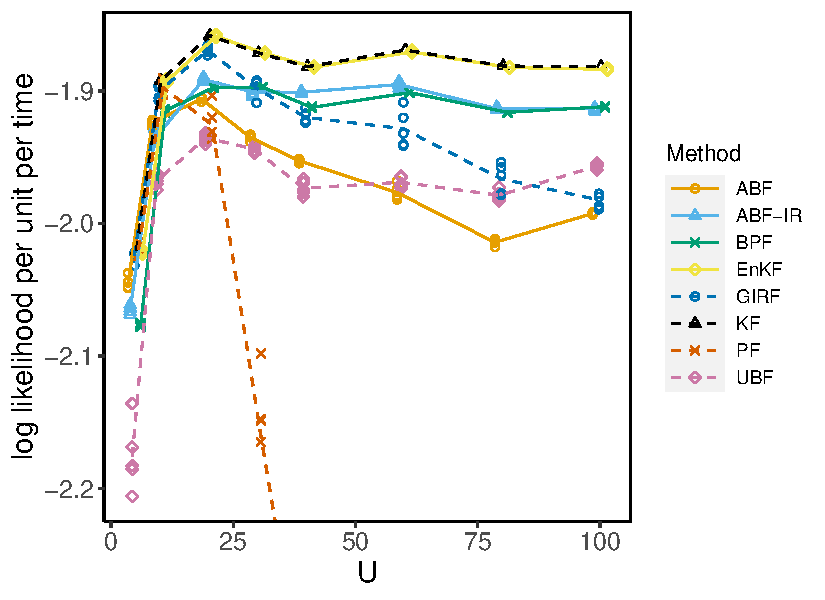
\includegraphics[width=10cm]{bm_alt_plot-1.pdf}

\vspace{-1mm}

$\cov\big(X_{\unit,\time}-X_{\unit,\time-1},X_{\altUnit,\time}-X_{\altUnit,\time-1}\big) \sim 0.4^{|\unit-\altUnit|}_{}$

\end{center}

\end{frame}

\begin{frame}
\frametitle{Filtering $U$ units of a coupled measles SEIR model}

\vspace{-3mm}

\begin{center}
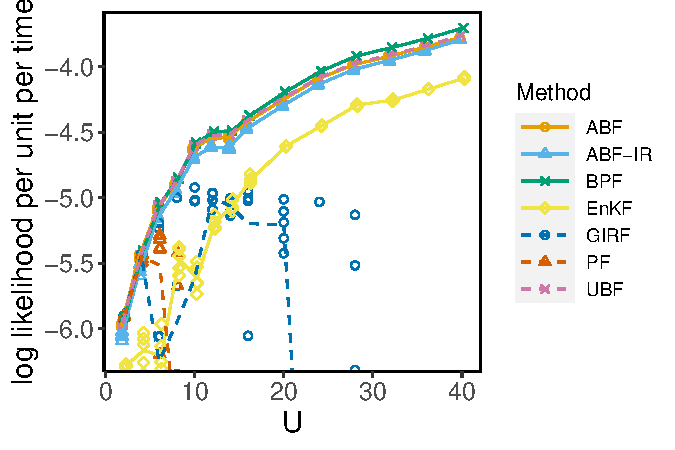
\includegraphics[width=10cm]{mscale_loglik_plot-1.pdf}


\end{center}

\vspace{-2mm}

Simulated data using a gravity model with geography, demography and transmssion parameters corresponding to UK pre-vaccination measles.

%\end{center}

\end{frame}


\begin{frame}
\frametitle{Filtering $U$ units of Lorenz 96 toy atmospheric model} 

\vspace{-3mm}

\begin{center}
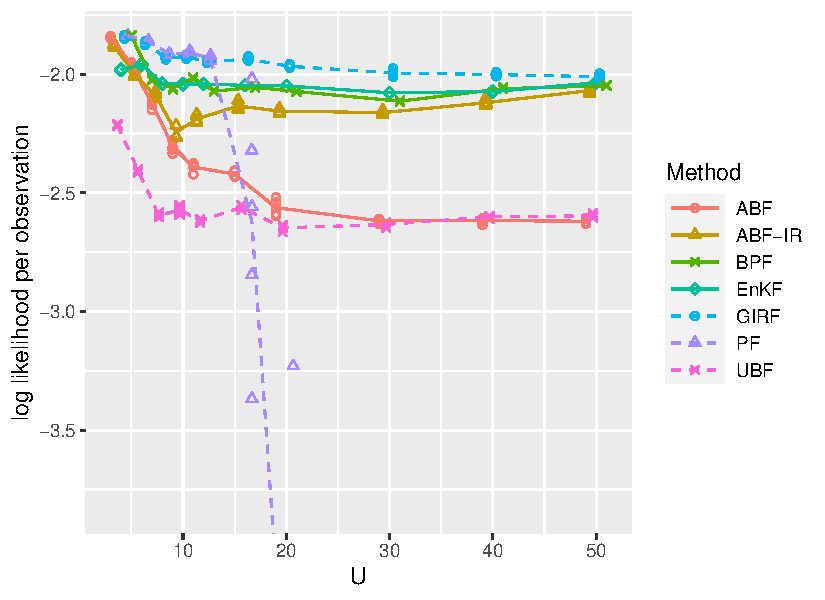
\includegraphics[width=10cm]{lz_loglik_plot-1.pdf}

\vspace{-1mm}

$dX_{\unit}(t) = \big \{  X_{\unit-1}(t) \big(X_{\unit+1}(t) - X_{\unit-2}(t)\big) - X_{\unit}(t) + F \big\} dt + \sigma \, dB_{\unit}(t)$

\end{center}

\end{frame}

\begin{frame}
\frametitle{From filtering to parameter inference}

\newcommand\inferencSep{\vspace{2.5mm}}

\begin{myitemize}
\item Log likelihood evaluation in principle enables likelihood-based or Bayesian inference.

\inferencSep

\item Iterated filtering for PF \citep{ionides15} and GIRF \citep{park20} maximizes the likelihood by randomly perturbing the parameters. 

\inferencSep

\item Particle Markov chain Monte Carlo can be applied with any likelihood estimate \citep{andrieu10}. It is numerically intractable when Monte Carlo estimates are costly and noisy.

\inferencSep

\item Iterated filtering is harder for bagged filters; it is possible but expensive \citep{ionides21}.

  \inferencSep
  
\item Iterated filtering works well for BPF when parameters are unit-specific, i.e., each city has its own parameters \citep{ning21-ibpf}.
It also can work with shared parameters (current unpublished work).

\end{myitemize}

\end{frame}

\begin{frame}{An iterated block particle filter for unit-specific parameters}


  \begin{center}
    
  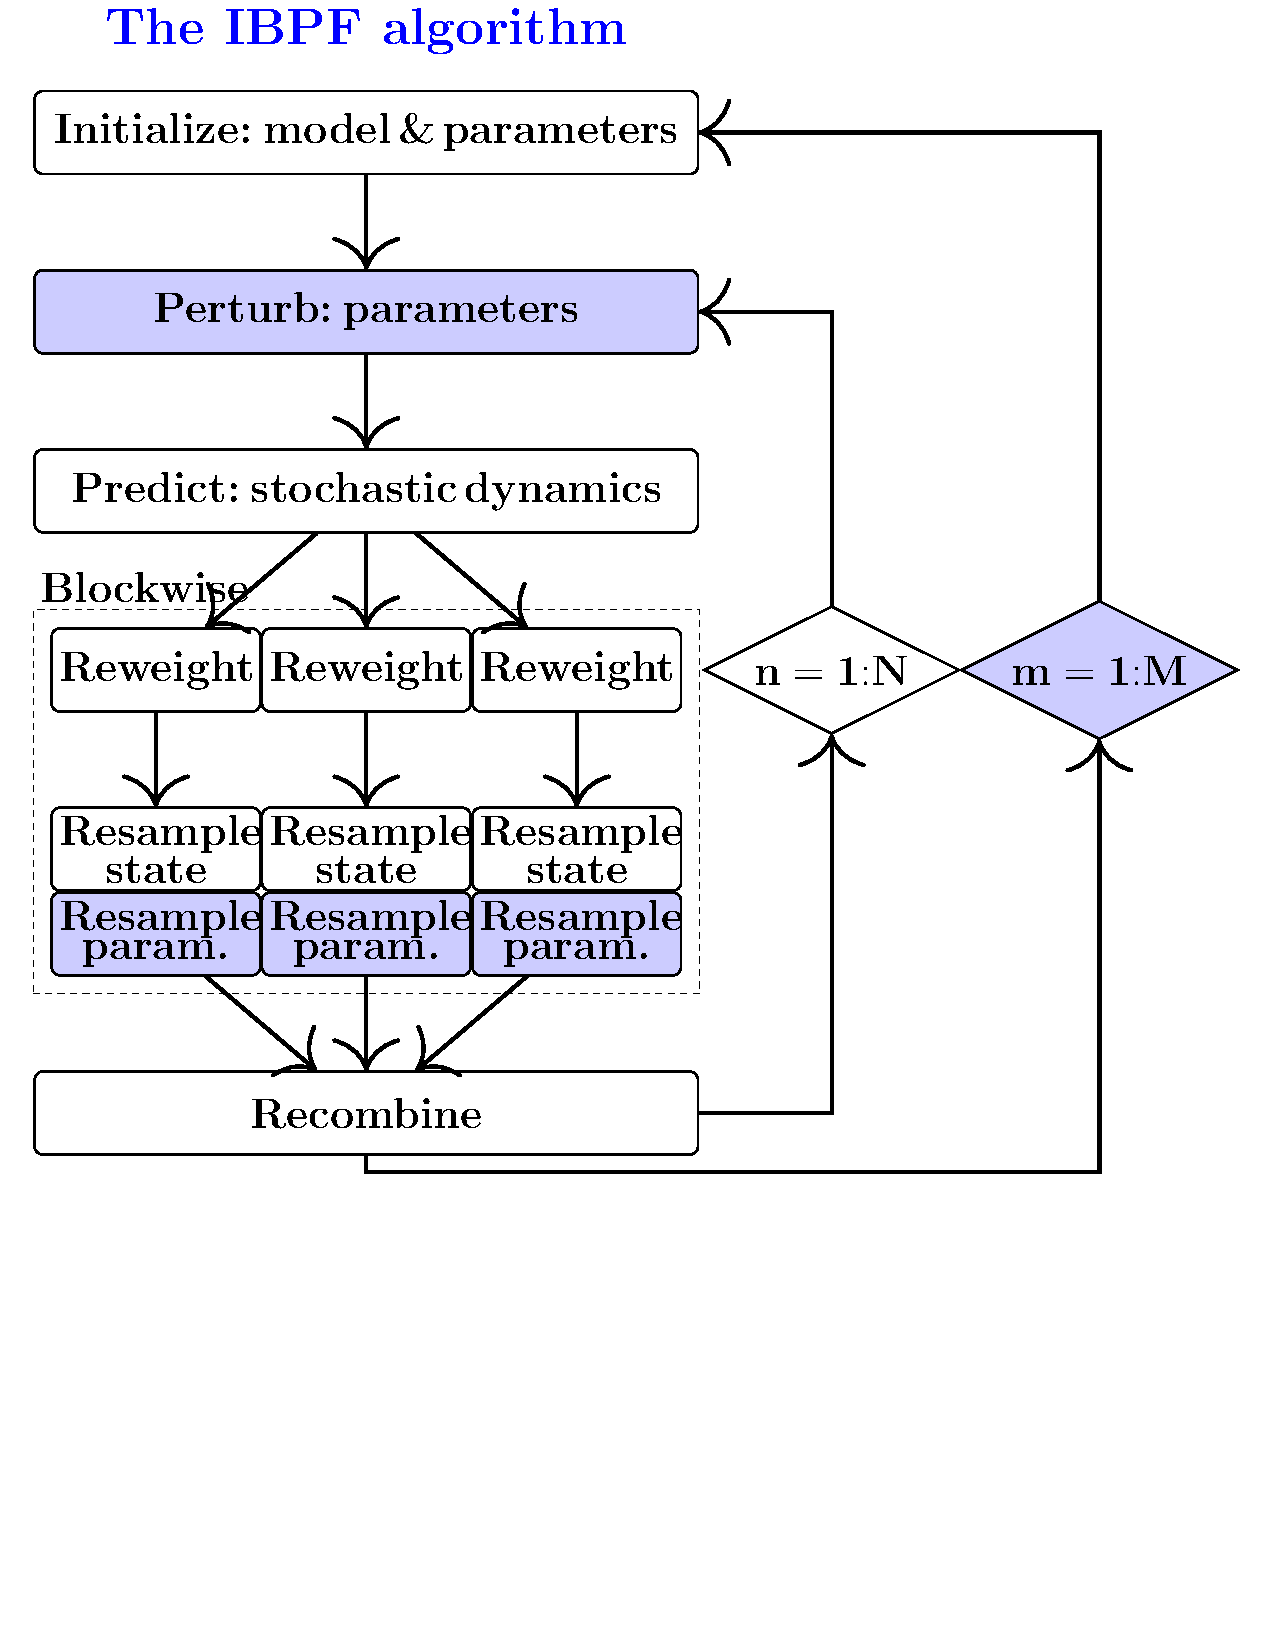
\includegraphics[trim={0 0 0 10mm},clip,width=9cm]{IBPF_workflow.pdf}


  \end{center}
  
\end{frame}


\begin{frame}

\frametitle{Measles likelihood slices for coupling parameter, $G$}

\vspace{-5mm}

\begin{columns}[T] % align columns
\begin{column}{.55\textwidth}
  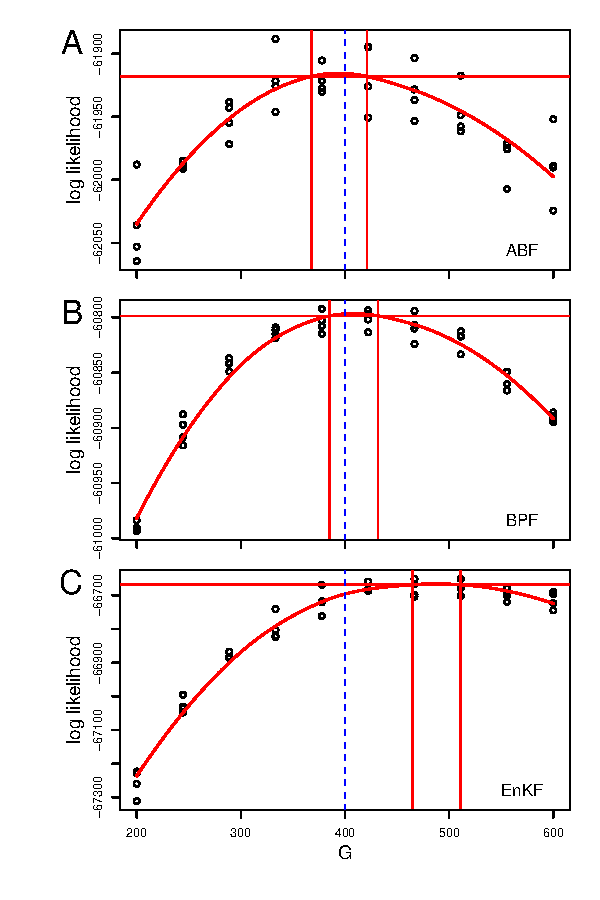
\includegraphics[width=6cm]{slice_combined_plot-1.pdf}
\end{column}
\begin{column}{.52\textwidth}

  \vspace{6mm}
  
  Simulating $15$ year of data from $U=40$ cities for the measles model.
  Slice likelihood, varying $G$ with other paramters fixed at the truth.

  \vspace{7mm}

  {\bf A}. Evaluation using ABF.

    \vspace{4mm}

  {\bf B}. Evaluation using BPF.

    \vspace{4mm}

  {\bf C}. Evaluation using EnKF.

  
\end{column}
\end{columns}

\end{frame}

\begin{frame}{Convergence of UBF, ABF \& ABF-IR \citep{ionides21}}
\begin{theorem}  \label{thm:tif}
Let $\MC{\loglik}$ denote the Monte Carlo likelihood approximation constructed by UBF, ABF or ABF-IR.
Consider a limit with a growing number of replicates, $\Rep\to\infty$.
Suppose regularity assumptions listed in the paper.
There are quantities $\el(\Unit,\Time) = O(1)$ and $V(\Unit,\Time)=O(\Unit^2\Time^2)$ such that
\begin{equation}
%\label{th1:lik:bound}
\nonumber
\Rep^{1/2}\big[ \MC{\loglik}-\loglik-\el\Unit\Time \big]  \xrightarrow[\Rep \rightarrow \infty]{d} \normal\big[0,V\big],
\end{equation}
where $\xrightarrow[\Rep \rightarrow \infty]{d}$ denotes convergence in distribution and $\normal[\mu,\Sigma]$ is the normal distribution with mean $\mu$ and variance $\Sigma$.
If an additional spatiotemporal mixing assumption holds, we obtain an improved variance bound
\begin{equation}
%\label{th1:lik:bound2}
\nonumber
%V < \ThmOneVarBound.
V(\Unit,\Time) = O(\Unit\Time)
\end{equation}
\end{theorem}
\end{frame}

\begin{frame}{Future work}

  \newcommand\futuresep{\vspace{3mm}}
  
  \begin{myitemize}
  \item We are getting close to the point where we can carry out likelihood-based inference for a flexible class of SpatPOMP models for measles.
Flexibility supports generation and testing of scientific hypotheses.
        
    \futuresep
    
  \item Measles was previously a motivating model system for POMP methods for single populations.

    \futuresep
    
    \item Many systems in ecology, epidemiology and elsewhere could be studied in a SpatPOMP framework \citep{bjornstad01}.
    
\end{myitemize}

\end{frame}

\begin{frame}[allowframebreaks]
\frametitle{References}
\bibliographystyle{apalike}
\bibliography{bib-sweden}
\end{frame}

\end{document}
